\documentclass{article}

\usepackage{graphicx}
\usepackage{tikz}
\usetikzlibrary{positioning,chains,fit,shapes,calc}
\newcommand{\indsize}{}
\newcommand{\colind}[2]{\displaystyle\smash{\mathop{#1}^{\raisebox{.5\normalbaselineskip}{\indsize #2}}}}
\newcommand{\rowind}[1]{\mbox{\indsize #1}}

\graphicspath{ {./images/} }

\begin{document}
        
\definecolor{myblue}{RGB}{80,80,160}
\definecolor{mygreen}{RGB}{80,160,80}

%Header
\begin{flushleft}
    Evan Wilcox\\
    CS1200 Fall 2018\\
    Homework 6\\
    Due: Monday 11/26/18
\end{flushleft}
        
%Problems
\begin{enumerate}

    %1
    \item Let R be the relation on $A$ and $B$ defined by aRb iff a divides b.

    \begin{enumerate}
        %a
        \item List the pairs in R.
        $$R=\{(2, 10), (3, 3), (3, 15), (3, 33), (5, -5), (5, 10), (5, 15)\}$$

        %b
        \item Represent the relation R as a 0,1-matrix.
        
        \begin{center}
            $\:\:\:B$
        \end{center}
        \[
            A \: \: \: \: \:
          \begin{array}{@{}c@{}}
            \rowind{2} \\ \rowind{3} \\ \rowind{4} \\ \rowind{5} \\ \rowind{6}
          \end{array}
          \mathop{\left[
          \begin{array}{ *{7}{c} }
             \colind{0}{-5}  &  \colind{0}{3}  &  \colind{0}{7}  & \colind{1}{10} & \colind{0}{15}  & \colind{0}{33} & \colind{0}{37}\\
             0 & 1 & 0 & 0 & 1 & 1 & 0 \\
             0 & 0 & 0 & 0 & 0 & 0 & 0 \\
             1 & 0 & 0 & 1 & 1 & 0 & 0 \\
             0 & 0 & 0 & 0 & 0 & 0 & 0
          \end{array}
          \right]}^{
          }
        \]
        
    \end{enumerate}
    %2
    \item R is symmetric but is not reflexive, antisymmetric or transitive.
    
    
    %3
    \item 
    \begin{enumerate}
        %a
        \item R is reflexive, symmetric and transitive but not antisymmetric.
        R is an equivalence relation but not a well order, partial order or 
        total order.

        %b
        \item Use python functions to verify your answers.\\
        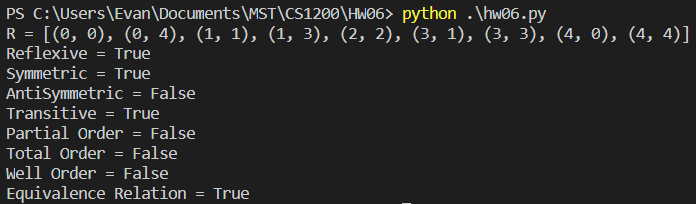
\includegraphics[scale=0.6]{3b3}\\
        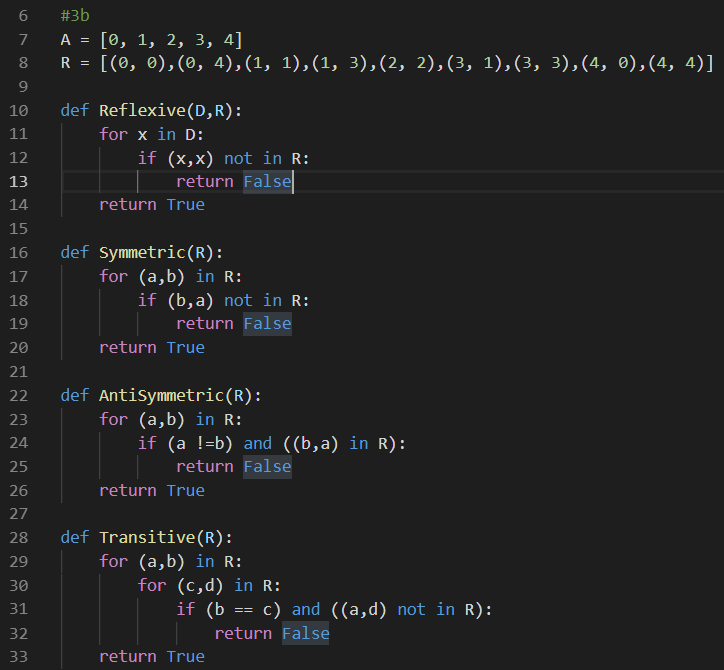
\includegraphics[scale=0.6]{3b1}\\
        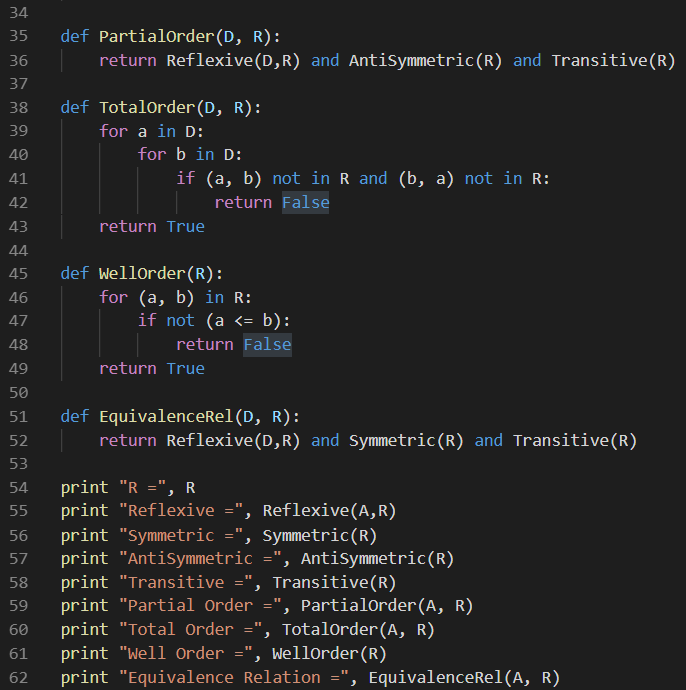
\includegraphics[scale=0.6]{3b2}
        

    \end{enumerate}

    \newpage
    %4
    \item 

    \begin{enumerate}
        %a
        \item Draw the directed graph representing R. If R can be represented by 
        an undirected graph, draw it.

        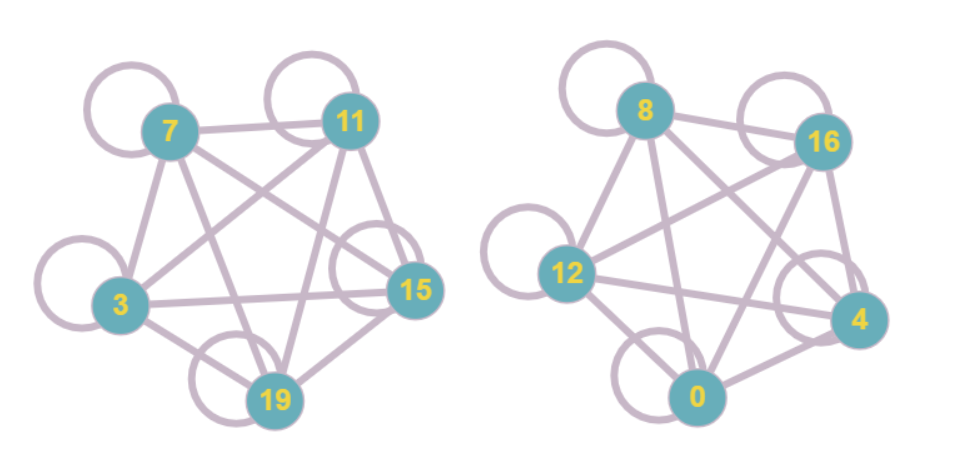
\includegraphics[scale=0.5]{4a1}\\
        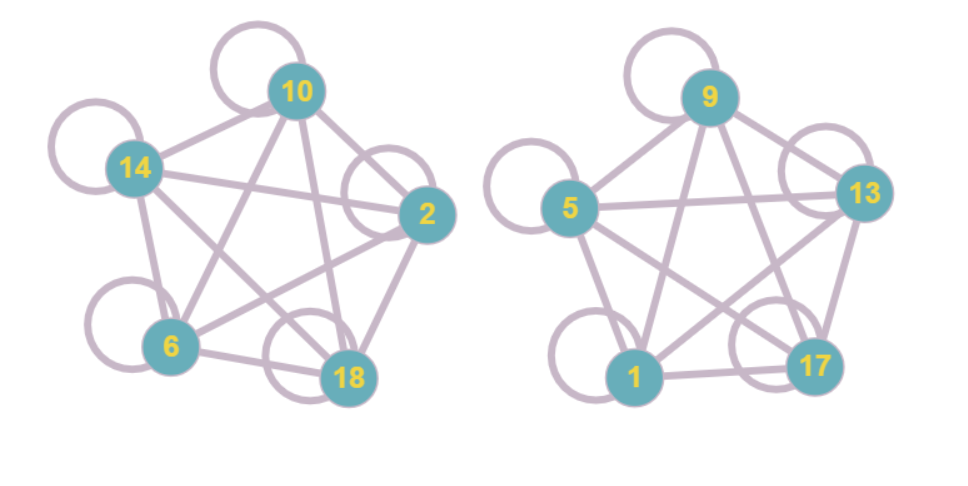
\includegraphics[scale=0.5]{4a2}
    
        \newpage
        %b
        \item Draw a 0,1-matrix to represent R with the rows and columns labeled.
        
        \begin{center}
            $\:\:\:\:\:\:\:\:\:\:\:\:B$
            \vspace{0.1cm}
        
        \[
            A \thinspace
          \begin{array}{@{}c@{}}
            \rowind{1}  \\ \rowind{2}  \\ \rowind{3}  \\ \rowind{4}  \\ \rowind{5}  \\
            \rowind{6}  \\ \rowind{7}  \\ \rowind{8}  \\ \rowind{9}  \\ \rowind{10} \\
            \rowind{11} \\ \rowind{12} \\ \rowind{13} \\ \rowind{14} \\ \rowind{15} \\
            \rowind{16} \\ \rowind{17} \\ \rowind{18} \\ \rowind{19} \\ \rowind{20} \\
          \end{array}
          \mathop{\left[
          \begin{array}{ *{20}{c} }
             \colind{1}{1}  &  \colind{0}{2}  & \colind{0}{3} & \colind{0}{4}  & \colind{1}{5} & \colind{0}{6} & \colind{0}{7}  &  \colind{0}{8}  &  \colind{1}{9}  & \colind{0}{10} & \colind{0}{11}  & \colind{0}{12} & \colind{1}{13} & \colind{0}{14}  &  \colind{0}{15}  &  \colind{0}{16}  & \colind{1}{17} & \colind{0}{18}  & \colind{0}{19} & \colind{0}{20}\\
             0 & 1 & 0 & 0 & 0 & 1 & 0 & 0 & 0 & 1 & 0 & 0 & 0 & 1 & 0 & 0 & 0 & 1 & 0 & 0\\
             0 & 0 & 1 & 0 & 0 & 0 & 1 & 0 & 0 & 0 & 1 & 0 & 0 & 0 & 1 & 0 & 0 & 0 & 1 & 0\\
             0 & 0 & 0 & 1 & 0 & 0 & 0 & 1 & 0 & 0 & 0 & 1 & 0 & 0 & 0 & 1 & 0 & 0 & 0 & 1\\
             1 & 0 & 0 & 0 & 1 & 0 & 0 & 0 & 1 & 0 & 0 & 0 & 1 & 0 & 0 & 0 & 1 & 0 & 0 & 0\\
             0 & 1 & 0 & 0 & 0 & 1 & 0 & 0 & 0 & 1 & 0 & 0 & 0 & 1 & 0 & 0 & 0 & 1 & 0 & 0\\
             0 & 0 & 1 & 0 & 0 & 0 & 1 & 0 & 0 & 0 & 1 & 0 & 0 & 0 & 1 & 0 & 0 & 0 & 1 & 0\\
             0 & 0 & 0 & 1 & 0 & 0 & 0 & 1 & 0 & 0 & 0 & 1 & 0 & 0 & 0 & 1 & 0 & 0 & 0 & 1\\
             1 & 0 & 0 & 0 & 1 & 0 & 0 & 0 & 1 & 0 & 0 & 0 & 1 & 0 & 0 & 0 & 1 & 0 & 0 & 0\\
             0 & 1 & 0 & 0 & 0 & 1 & 0 & 0 & 0 & 1 & 0 & 0 & 0 & 1 & 0 & 0 & 0 & 1 & 0 & 0\\
             0 & 0 & 1 & 0 & 0 & 0 & 1 & 0 & 0 & 0 & 1 & 0 & 0 & 0 & 1 & 0 & 0 & 0 & 1 & 0\\
             0 & 0 & 0 & 1 & 0 & 0 & 0 & 1 & 0 & 0 & 0 & 1 & 0 & 0 & 0 & 1 & 0 & 0 & 0 & 1\\
             1 & 0 & 0 & 0 & 1 & 0 & 0 & 0 & 1 & 0 & 0 & 0 & 1 & 0 & 0 & 0 & 1 & 0 & 0 & 0\\
             0 & 1 & 0 & 0 & 0 & 1 & 0 & 0 & 0 & 1 & 0 & 0 & 0 & 1 & 0 & 0 & 0 & 1 & 0 & 0\\
             0 & 0 & 1 & 0 & 0 & 0 & 1 & 0 & 0 & 0 & 1 & 0 & 0 & 0 & 1 & 0 & 0 & 0 & 1 & 0\\
             0 & 0 & 0 & 1 & 0 & 0 & 0 & 1 & 0 & 0 & 0 & 1 & 0 & 0 & 0 & 1 & 0 & 0 & 0 & 1\\
             1 & 0 & 0 & 0 & 1 & 0 & 0 & 0 & 1 & 0 & 0 & 0 & 1 & 0 & 0 & 0 & 1 & 0 & 0 & 0\\
             0 & 1 & 0 & 0 & 0 & 1 & 0 & 0 & 0 & 1 & 0 & 0 & 0 & 1 & 0 & 0 & 0 & 1 & 0 & 0\\
             0 & 0 & 1 & 0 & 0 & 0 & 1 & 0 & 0 & 0 & 1 & 0 & 0 & 0 & 1 & 0 & 0 & 0 & 1 & 0\\
             0 & 0 & 0 & 1 & 0 & 0 & 0 & 1 & 0 & 0 & 0 & 1 & 0 & 0 & 0 & 1 & 0 & 0 & 0 & 1\\
          \end{array}
          \right]}^{
          }
        \]
        \end{center}
        %c
        \item R is an equivalence relation but not a partial order, total order or well order.
        
    \end{enumerate}

    \newpage
    %5
    \item 
    
    \begin{enumerate}
        %a
        \item Draw a bipartite graph representation of f.

        \begin{tikzpicture}[thick,
            every node/.style={draw,circle},
            fsnode/.style={fill=myblue},
            ssnode/.style={fill=mygreen},
            every fit/.style={ellipse,draw,inner sep=-2pt,text width=2cm},
            ->,shorten >= 3pt,shorten <= 3pt
            ]
          
            % the vertices of A
            \begin{scope}[start chain=going below,node distance=5mm]
            \foreach \i in {0,1,2,...,5}
                \node[fsnode,on chain] (f\i) [label=left: \i] {};
            \end{scope}
            
            % the vertices of f(A)
            \begin{scope}[xshift=4cm,yshift=-0.0cm,start chain=going below,node distance=5mm]
            \foreach \i in {0,1,2,...,5}
                \node[ssnode,on chain] (s\i) [label=right: \i] {};
            \end{scope}
            
            % the set U
            \node [black,fit=(f0) (f5),label=above:$A$] {};
            % the set V
            \node [black,fit=(s0) (s5),label=above:$f(A)$] {};
            
            % the edges
            \draw (f0) -- (s5);
            \draw (f1) -- (s3);
            \draw (f2) -- (s0);
            \draw (f3) -- (s0);
            \draw (f4) -- (s4);
            \draw (f5) -- (s1);
        \end{tikzpicture}

        %b
        \item f is not an injection, surjection, or bijection.

        \newpage
        %c
        \item Write a Python program to test whether the functions are 
        injections, surjections, or bijections.

        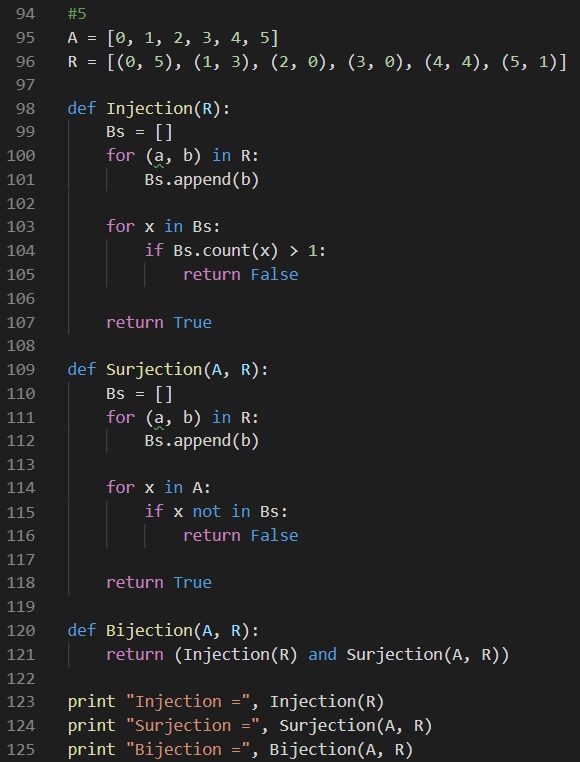
\includegraphics[scale=0.7]{5c1}\\
        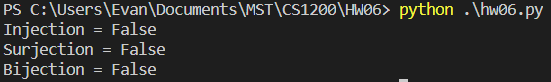
\includegraphics[scale=0.7]{5c2}

    \end{enumerate}

    \newpage
    %6
    \item
    \begin{enumerate}
        %a
        \item Write the formulas for $g\circ f$ and $f\circ g$.
        $$g\circ f = 12n+9$$
        $$f\circ g = 12n+5$$

        %b
        \item Determine whether each of $f, g, g\circ f, f\circ g$ are injections, 
        surjections or bijections.

        \begin{center}
        \begin{tabular}{ |c|c|c|c| }
            \hline
            Function & injection? & surjection? & bijection?\\
            \hline
            $f$ & Yes & Yes & Yes\\
            \hline
            $g$ & Yes & Yes & Yes\\
            \hline
            $g\circ f$ & Yes &Yes  & Yes\\
            \hline
            $f\circ g$ & Yes & Yes & Yes\\
            \hline
        \end{tabular}
        \end{center}

        %c
        \item Compute $(f\circ g)^{-1}(\{-5, -3, 0, 7, 9, 21, 22, 23, 45\})$ 
        and $(g\circ f)^{-1}(\{-7, 0, 5, 7, 9, 17, 22, 41\})$.

        \begin{center}
        \begin{tabular}{ c|c|c|c|c|c|c|c|c|c}
            n &-5 & -3 & 0 & 7 & 9 & 21 & 22 & 23 & 45\\
            \hline
            $(f\circ g)^{-1}(n)$ & $-\frac{5}{6}$ & $-\frac{2}{3}$ & $-\frac{5}{12}$ & $\frac{1}{6}$ & $\frac{1}{3}$ & $1\frac{1}{3}$ & $1\frac{5}{12}$ & $1\frac{1}{2}$ & $3\frac{1}{3}$\\
        \end{tabular}
        \end{center}

        \begin{center}
        \begin{tabular}{ c|c|c|c|c|c|c|c|c}
            n & -7 & 0 & 5 & 7 & 9 & 17 & 22 & 41\\
            \hline
            $(g\circ f)^{-1}(n)$ & $-1\frac{1}{3}$ & $-\frac{3}{4}$ & $-\frac{1}{3}$ & $-\frac{1}{6}$ & 0 & $\frac{2}{3}$ & $1\frac{1}{12}$ & $2\frac{2}{3}$\\
        \end{tabular}
        \end{center}

    \end{enumerate}

    \vspace{4cm}
    %7
    \item Let $N$ be the set of natural numbers and $f:N \rightarrow N$ 
    be the function $f(n) = 5n+4$. 

    \begin{center}
    \begin{tabular}{ c|c|c|c|c|c|c|c|c|c|c|c}
        n & 4 & 5 & 8 & 9 & 10 & 11 & 13 & 14 & 15 & 24 & 30\\
        \hline
        $f^{-1}(n)$ & 0 & $\frac{1}{5}$ & $\frac{4}{5}$ & 1 & $1\frac{1}{5}$ & $1\frac{2}{5}$ & $1\frac{4}{5}$ & 2 & $2\frac{1}{5}$ & 4 & $5\frac{1}{5}$
    \end{tabular}
    \end{center}
\end{enumerate}

\end{document}